\section{Materials and methods}

% En estos capítulos, es necesario describir:
% •	los aspectos más relevantes del diseño y desarrollo del trabajo
% •	la metodología elegida para realizar este desarrollo, describiendo las alternativas posibles, las decisiones tomadas, y los criterios utilizados para tomar estas decisiones.
% •	descripción de los productos obtenidos.
 
% La estructuración de los capítulos puede variar en función del tipo de trabajo.  
 
% En caso de que proceda, se incluirá un apartado de “Valoración económica del trabajo”. Este apartado indicará los gastos asociados al desarrollo y mantenimiento del trabajo, así como los beneficios económicos obtenidos y un análisis final sobre la viabilidad del producto.

\subsection{Data Acquisition}

\subsubsection{Mouse MSI-1 and MSI-1's RMM1}

\href{https://www.uniprot.org/}{\texttt{Uniprot}'s database} was consulted for the structure of the mouse MSI-1 protein (see \textbf{Figure \ref{fig:Q61474uniprot}}). Unfortunately, there was no NMR crystal structure for the complete protein: the only available complete structure was \texttt{AlphaFold}'s prediction of the structure (see \textbf{Figure \ref{fig:3DMSI}}). Said structure had low confidence in the aminoacid sequence not corresponding to the RRMs. Therefore, the crystal structure of MSI-1's RRM1 (see \textbf{Figure \ref{fig:3DRRM1}}) was to be employed instead for the docking simulations.

\begin{figure}[htbp!]
    \centering
    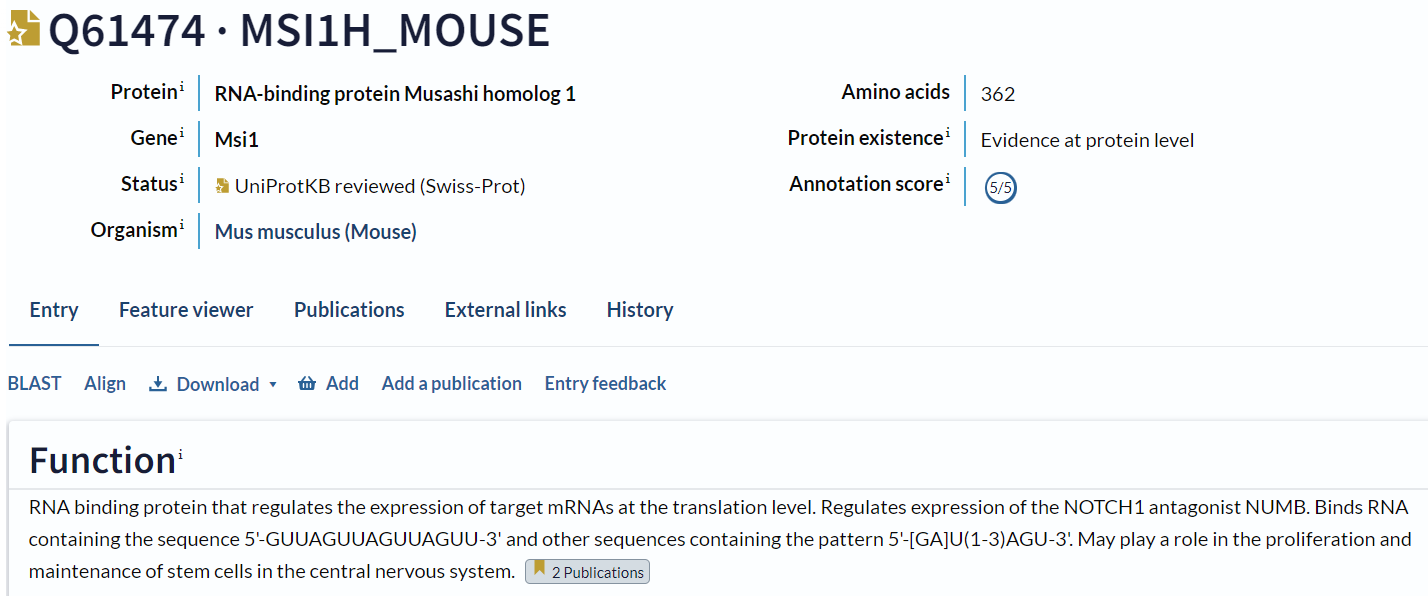
\includegraphics[width=\linewidth]{assets/Q61474_uniprot_entry.png}
    \caption{\href{https://www.uniprot.org/uniprotkb/Q61474/entry}{Uniprot entry Q61474} corresponding to the mouse MSI-1. Screenshot taken on 08/01/2023.}
    \label{fig:Q61474uniprot}
\end{figure}

The crystal NMR structure was downloaded as a \texttt{.pdb} file.

\subsubsection{Fatty acids}

The fatty acids to be employed down the line in the docking simulations were retrieved from their respective \href{https://www.chemspider.com/}{\texttt{Chemspider}} entries. The fatty acids downloaded were:

\begin{itemize}
    \item\href{https://www.chemspider.com/Chemical-Structure.392692.html}{arachidonic acid}
    \item\href{https://www.chemspider.com/Chemical-Structure.4444105.html}{linoleic acid}
    \item\href{https://www.chemspider.com/Chemical-Structure.393217.html}{oleic acid}
    \item\href{https://www.chemspider.com/Chemical-Structure.960.html}{palmitic acid}
    \item\href{https://www.chemspider.com/Chemical-Structure.5091.html}{stearic acid}
\end{itemize}

The molecules are shown in \textbf{Figure \ref{fig:fatty_acids}}.

\begin{figure}[htbp!]
    \centering
    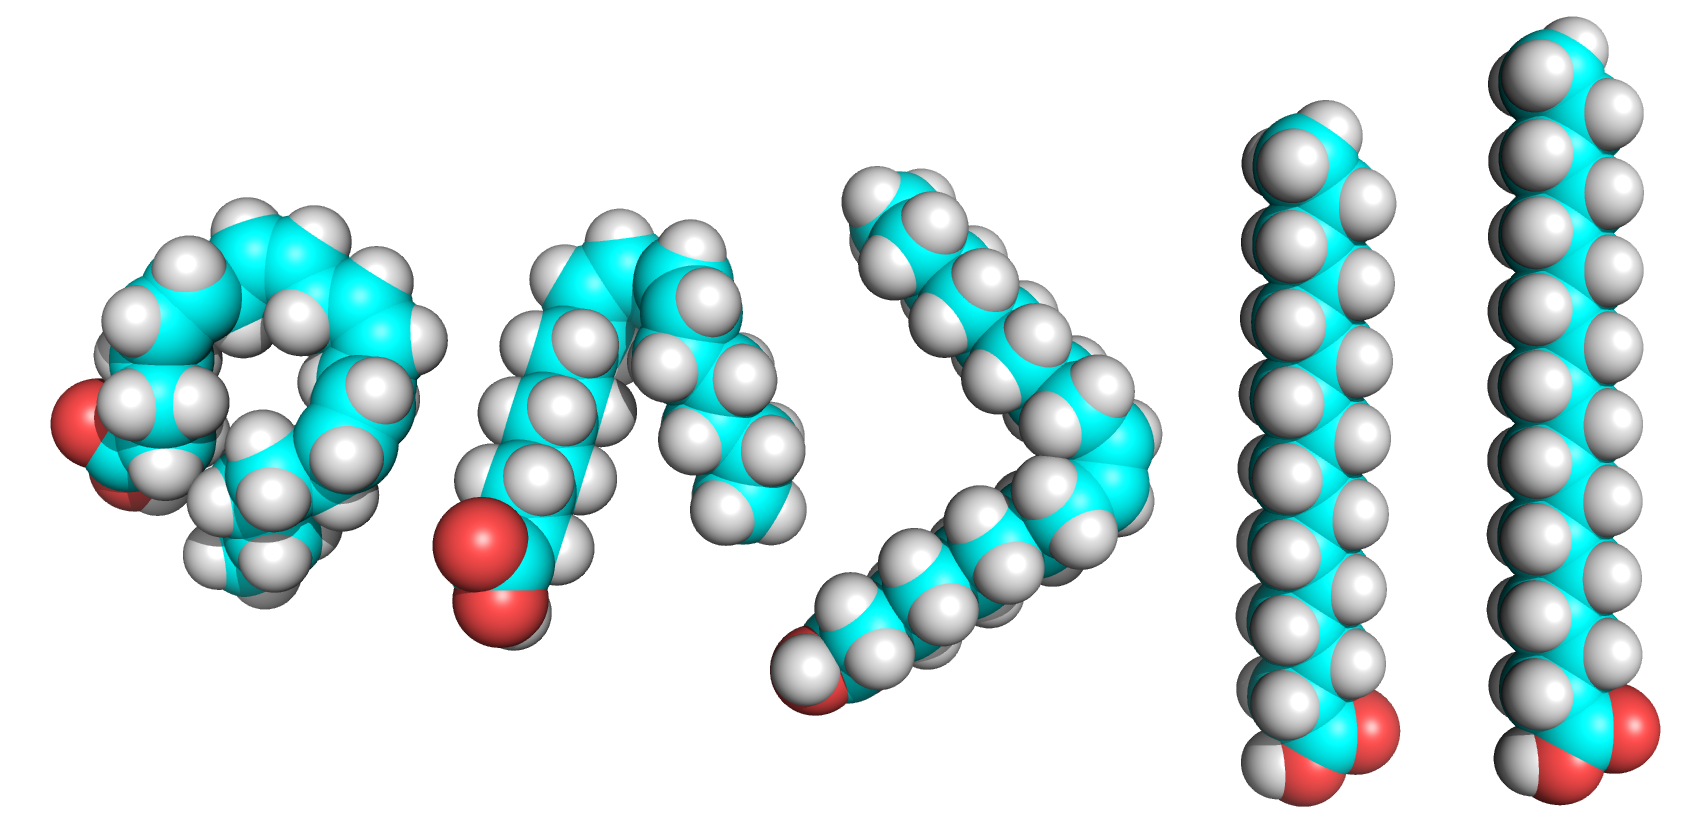
\includegraphics[width=0.75\linewidth]{assets/fatty_acids.png}
    \caption{3D structure of the fatty acids to be employed. From left to right: arachidonic acid, linoleic acid, oleic acid, palmitic acid and stearic acid. Colors represent the atoms present in the structures: cyan is Carbon, red is Oxygen and white is Hydrogen. Visualized through \href{https://pymol.org/2/}{\texttt{Pymol}}.}
    \label{fig:fatty_acids}
\end{figure}

The molecules' 3D structures were downloaded as \texttt{.mol} files. 

\subsection{Generation of 3D RNA molecule structures}

The raw RNA sequences to be employed were retrieved from \cite{dolcemascolo_2022} and are shown in \textbf{\nameref{appendix_A}}, where they crafted small RNA oligos based on a the selex optimal RNA sequence. RNA takes specific spatial conformations when in aqueous media, be it \textit{in vitro} or \textit{in vivo}, which can be computed directly from the RNA sequence by means of pre-measured experimental parameters \cite{santalucia_1998}.\\

To do so, the Nupack software was employed \cite{dirks_2004} (specifically its associated \texttt{Python} package) and the structures in dot-bracket notation\footnote{Dot-bracket notation is a simplistic manner of representing DNA or RNA secondary structure. For more details, see \cite{rna_structure_notations}.} were recorded. In addition, the sequences were subjected to pairwise alignments (by means of MAFFT \cite{katoh_2002}) to highlight the mutations present with respect to the original oligo. The \texttt{Python} script employed to perform these computations is found in \textbf{\nameref{appendix_B}}.

\vfill

\pagebreak

The results are shown in \textbf{Figure \ref{fig:dataset}}:

\begin{figure}[htbp!]
    \lstinputlisting[basicstyle=\tiny]{assets/dataset.tsv}
    \caption{RNA sequences along with the result of the pairwise alingments and Nupack's prediction of their secondary structure.}
    \label{fig:dataset}
\end{figure}

With this information (RNA sequence and secondary structure), the 3D conformation of each of the RNA motifs was computed by means of the \href{https://rnacomposer.cs.put.poznan.pl/}{\texttt{RNAComposer}} web server \cite{biesiada_2016} and downloaded in \texttt{.pdb} format. The corresponding 3D structures of the RNA motifs are shown in \textbf{Figure \ref{fig:RNAs}}.

\begin{figure}[htbp!]
    \centering
    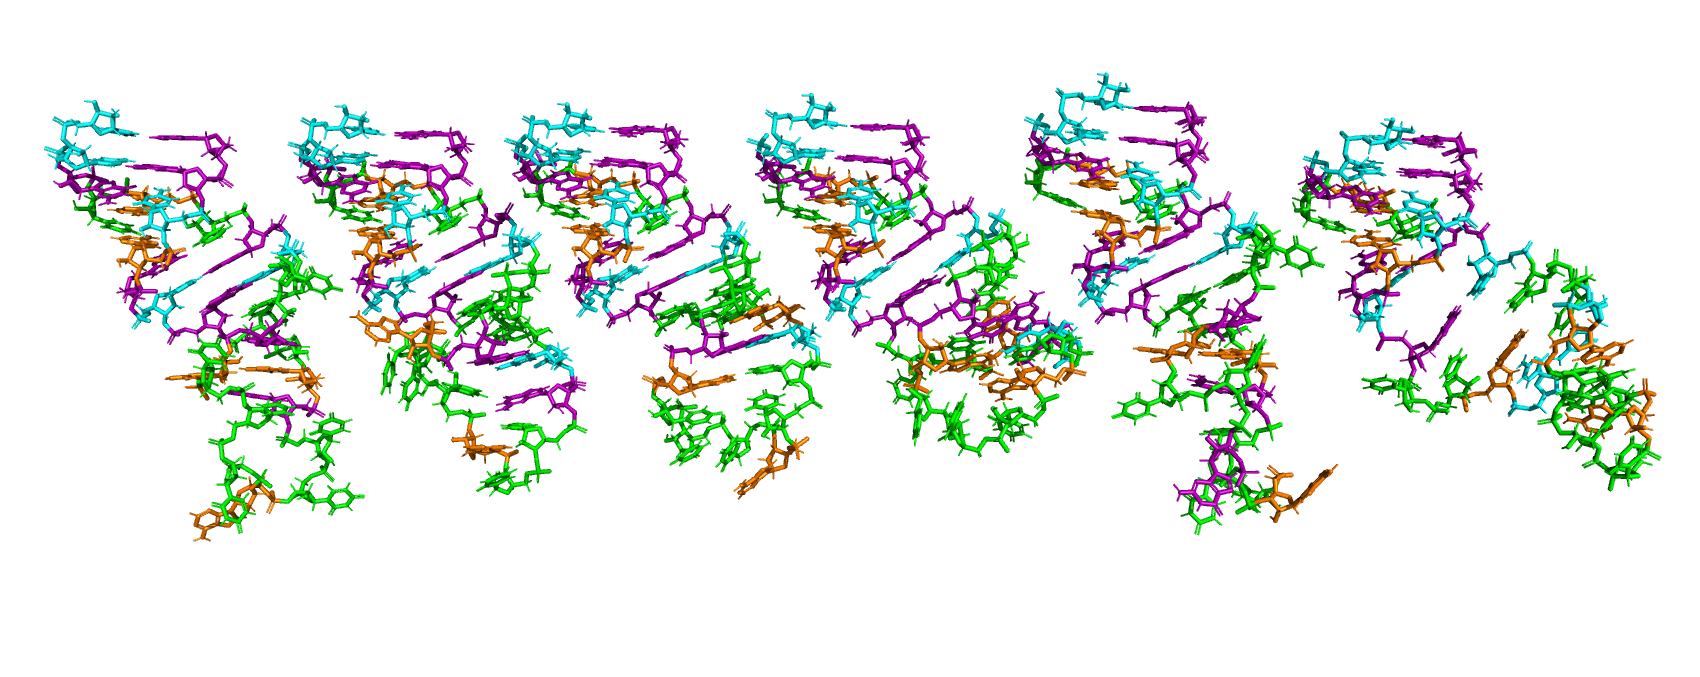
\includegraphics[width=\linewidth]{assets/RNAs.png}
    \caption{3D structures of the RNA motifs. From left to right: the original RNA motif followed by the 5 mutants. Colors represent the nucleotidic bases: orange is Adenine, purple is Guanine, cyan is Cytosine and green is Uracil. Visualized through \href{https://pymol.org/2/}{\texttt{Pymol}}.}
    \label{fig:RNAs}
\end{figure}

With the 3D structures of the RNA motifs, the next step is to prepare the protein-RNA docking simulations.

\subsection{Protein-RNA docking simulations with \texttt{LightDock}}

For the protein-RNA docking simulations, the \texttt{LightDock} \cite{jimenez_garcia_2017} docking software was chosen. The main reasons are the simplicity of \texttt{LightDock}, the quality of the documentation and that the software is written in \texttt{Python}, which eases debugging steps in case of complications. Originally, \texttt{LightDock} was not meant for protein-RNA docking simulations. However, by means of some reasearch and auxiliary \texttt{Python} scripts, a simple and novel pipeline was designed which makes it possible to perform such docking simulations with \texttt{LightDock}. This pipeline takes inspiration on the \href{https://lightdock.org/tutorials/0.9.3/dna_docking}{protein-DNA example tutorial from the \texttt{LightDock} documentation}.

\subsubsection{Protein preparation}

First, MSI-1's RRM1 \texttt{.pdb} file needs to have their hydrogen atoms modified and relabeled so that they match the \texttt{AMBER94} force field, which is the parameter set that is going to be used in this docking simulation. To do so, the softwares \href{https://github.com/rlabduke/reduce}{\texttt{REDUCE}} and \href{https://github.com/haddocking/pdb-tools/}{\texttt{PDB-Tools}} \cite{rodrigues_2018} were employed.\\

In addition, the MSI-1's RRM1 \texttt{.pdb} file needed an additional motification related to the \texttt{AMBER94} force field: regular \texttt{.pdb} files employ the \texttt{HIS} identifier for the Histidine aminoacid, which does not appear in the \texttt{AMBER94} force field. The reason behind this is that for the \texttt{AMBER94} force field, Histidine can be one of 3 possible residues \cite{amber_histidine}:

\begin{enumerate}
    \item\texttt{HID}: Histidine with a single hydrogen on the delta nitrogen
    \item\texttt{HIE}: Histidine with a single hydrogen on the epsilon nitrogen
    \item\texttt{HIP}: Histidine with hydrogens on both nitrogens (delta and epsilon). This Histidine has a positive charge
\end{enumerate}

Therefore, one has to check which kind of Histidine residue is present in the molecule, and change it for the corresponding \texttt{AMBER94}-compatible identifier. This can be done with a simple \texttt{Python} script, which is found in \textbf{\nameref{appendix_C}}.

\subsubsection{RNA preparation}


% Las siguientes subsecciones son la liada parda que aún he de arreglar
\subsection{Fatty acid-protein docking simulations}
\subsection{Fatty acid-protein-RNA docking simulations}


%• Docking simulations will be carried out with LightDock (https://lightdock.org/), and the subsequent results will be visualized with the open source version of PyMol (https://github.com/schrodinger/pymol-open-source). 


%     \begin{itemize}
%         \item La librería \texttt{proDy} (una librería que emplea \texttt{lightdock} para las simulaciones de docking) no reconoce cadenas de RNA expecificadas en los ficheros \texttt{.pdb} si estas son especificadas mediante el prefijo \texttt{R} en los identificadores de las bases nucleotídicas (es decir, \texttt{RA}, \texttt{RG}, \texttt{RU} y \texttt{RC}) en la estructura de la molécula. Este hecho resulta en un error en el paso de setup de \texttt{lightdock}.
    
%         La mitigación de este problema consistió en crear un script de \texttt{Python} que elimina ese prefijo \texttt{R} de los ficheros \texttt{.pdb}. Este script se encuentra en \textbf{\nameref{anexo_A}}.
    
%         \item Las simulaciones de docking no funcionaban puesto que el RNA tenía conflictos con los parámetros del AMBER \textit{force field}. Esto se debe a que los parámetros que \texttt{lightdock} debía usar para RNA, se especifican precisamente con el prefijo \texttt{R} eliminado en la mitigación anterior. Por lo tanto, la mitigación de este problema consiste en volver a añadir el prefijo \texttt{R} a los ficheros \texttt{.pdb} mediante un script de \texttt{Python}. Este script se encuentra en \textbf{\nameref{anexo_B}}.
    
%         \item Pese a la mitigación anterior, las simulaciones continuaban fallando. Esto se debía a que los RNAs empleados terminan en ``OH'' en los extremos 3' y 5'. \texttt{lightdock} no reconoce estos átomos como parte de la estructura ni tiene parámetros de AMBER \textit{force field} para ellos. Como mitigación, he decidido eliminar esos átomos mediante un script de \texttt{Python}. Asumo que eliminar un par átomos en los extremos de la molécula de RNA no marca mucha diferencia a la hora de hacer el docking. Este script se encuentra en \textbf{\nameref{anexo_C}}.
    

%         \item Con las mitigaciones anteriores, \texttt{lightdock} ejecutó sin problemas. Sin embargo, \texttt{lgd\_generate\_conformations} no ejecutó correctamente a la hora de construir los modelos de docking en formato \texttt{.pdb}. Esto se debe a que \texttt{lgd\_generate\_conformations}, como en uno de los pasos anteriores, no reconocía la estructura de RNA por el prefijo de la \texttt{R}. Por ende, hubo que añadir un paso de eliminación de ese prefijo de la \texttt{R}. Esto se llevó a cabo mediante el script de \texttt{Python} encontrado en \textbf{\nameref{anexo_A}}.

%     \end{itemize}

%     Con esas mitigaciones, los dockings se ejecutaron sin problema. Resolver las anteriores complicaciones implicaron una mayor inversión de tiempo en la parte de docking de este trabajo. Este hecho, y tras consultarlo con el supervisor de este trabajo, llevó a desechar la parte de dinámica molecular por completo.

%     \item El objetivo 4 no se ha completado puesto que no se había contemplado para este período de tiempo. Las simulaciones de docking con los ácidos grasos están siendo ejecutadas durante la escritura de este informe.

% \end{itemize}

% \section{Relación de las actividades realizadas}

% \subsection{Actividades previstas en el plan de trabajo}

% Las actividades llevadas a cabo son las siguientes:

% \begin{enumerate}
%     \item Creación de los scripts de \texttt{Python} mencionados en las mitigaciones anteriores.

%     \item Ejecución de las simulaciones de docking siguientes:
%     \begin{itemize}
%         \item MSI-1 y el motivo de RNA original
%         \item MSI-1 y el motivo de RNA original (con estructura lineal)
%         \item MSI-1 y el mutante de RNA número 1
%         \item MSI-1 y el mutante de RNA número 2
%         \item MSI-1 y el mutante de RNA número 3
%         \item MSI-1 y el mutante de RNA número 4
%         \item MSI-1 y el mutante de RNA número 5
%     \end{itemize}

%     \item Selección de los 10 modelos de docking con mejor score de luciferina para cada una de las simulaciones mencionadas anteriormente.

%     \item Visualización de los modelos generados por \texttt{lightdock} mediante \texttt{pymol}.

%     Los resultados se encuentran en los siguientes anexos:
%     \begin{itemize}
%         \item\textbf{\nameref{anexo_E}}
%         \item\textbf{\nameref{anexo_F}}
%         \item \textbf{\nameref{anexo_G}}
%         \item \textbf{\nameref{anexo_H}}
%         \item \textbf{\nameref{anexo_I}}
%         \item \textbf{\nameref{anexo_J}}
%         \item \textbf{\nameref{anexo_K}}
%         \item \textbf{\nameref{anexo_L}}
%         \item \textbf{\nameref{anexo_M}}
%         \item \textbf{\nameref{anexo_N}}
%         \item \textbf{\nameref{anexo_O}}
%     \end{itemize}

% \end{enumerate}

% \subsection{Actividades no previstas y realizadas o programadas}

% Adicionalmente, se llevaron las siguientes actividades no previstas:

% \begin{itemize}

%     \item Se llevó a cabo la creación de un script de \texttt{Python} cuyo objetivo es añadir la estructura secundaria de la proteína MSI-1 a los modelos de docking (dado que \texttt{lightdock} elimina esa información).

%     \item Se inició una conversación con el equipo desarrollador de \texttt{lightdock} con el objetivo de elaborar un tutorial para el caso de docking proteína-RNA basado en este trabajo.

% \end{itemize}


% \item El objetivo 2 no se ha cumplido debido a unas complicaciones a la hora de hacer el docking proteína-RNA en el programa \texttt{lightdock}. 
    
% Varios intentos de \textit{setup} y simulación de docking fallaban sin motivo aparente. Tras varios intentos, descubrí que el problema se debía a que la protonación de los ficheros \texttt{.pdb} correspondientes a los motivos de RNA y el fichero \texttt{.pdb} del RRM1 de la proteína MSI-1 eran incompatibles. La mitigación es aparentemente sencilla y consiste en los siguientes pasos:

% \begin{itemize}
%     \item Emplear el software \href{https://github.com/rlabduke/reduce}{\texttt{reduce}} para corregir la protonación en los ficheros \texttt{.pdb}.
%     \item Emplear el software \href{https://github.com/haddocking/pdb-tools/}{\texttt{pdb-tools}} para corregir la numeración de los átomos en los ficheros \texttt{.pdb}.
%     \item Controlar que los protones corregidos por \texttt{reduce} a las estructuras de RNA sean 100\% compatibles con el campo de fuerzas \texttt{AMBER94} (que es el que se emplea como función \texttt{score} cuando se realiza docking con ácidos nucleicos). La documentación de \texttt{lightdock} proporciona un script para llevar a cabo este control: \href{https://lightdock.org/tutorials/0.9.1/dna_docking/data/reduce_to_amber.py}{\texttt{reduce\_to\_amber.py}}.
% \end{itemize}

% En principio, una vez llevados a cabo estos pasos, las simulaciones de docking pueden llevarse a cabo con normalidad. Por lo tanto, es necesario la descarga del software mencionado anteriormente.

% \item El objetivo 3 no se ha completado puesto que no se había contemplado para este período de tiempo. Sin embargo, he tenido que llevar a cabo un cambio fundamental que afecta el cumplimiento de este objetivo. Originalmente, el plan de trabajo contemplaba que las simulaciones de dinámica mulecular se llevasen a cabo con el software \href{https://ambermd.org/}{\texttt{Amber}}. Sin embargo, en contraste con mi estudio inicial durante la elaboración del plan de trabajo, \texttt{Amber} requiere una licencia de pago. Por lo tanto, siguiendo una de las mitigaciones propuestas en el plan de trabajo, las simulaciones de dinámica molecular se llevarán a cabo con \href{http://www.biomolecular-modeling.com/Abalone/}{\texttt{Abalone II}}.

% Las actividades llevadas a cabo son las siguientes:

% \begin{enumerate}
%     \item Diseño de 5 mutantes para el motivo de RNA reconocido por la proteína MSI-1. Para la obtención del motivo de RNA \texttt{wild-type} que interacciona con la proteína MSI-1, se acudió a los trabajos \cite{imai_2001} y \cite{clingman_2014}. Sin embargo, este motivo existe en un contexto de secuencia adicional que permite su correcto plegamiento a una estructura secundaria reconocida por MSI-1. Por ello, siguiendo el ejemplo de \cite{dolcemascolo_2022}, se añadieron una serie de ácidos nucleicos alrededor del motivo de reconocimiento para que el plegamiento predicho de la secuencia de RNA fuese como en las referencias \cite{imai_2001} y \cite{clingman_2014}. La estructura secundaria del plegamiento de la secuencia de RNA fue comprobada mediante \href{http://www.nupack.org/}{\texttt{Nupack}}.
%     \item Mediante la secuencia de RNA resultante, se generaron 5 mutantes mediante sustituciones e inserciones de bases nucleotídicas. Los mutantes candidatos fueron seleccionados según su estructura secundaria, comprobada mediante \texttt{Nupack}. Las secuencias finales se encuentran en el \textbf{\nameref{anexo_A}}.
%     \item Las secuencias mencionadas anteriormente fueron tabuladas, y se añadieron el resultado del alineamiento con la secuencia original y la estructura secundaria (en formato \texttt{dot-bracket}). Esta tabla se encuentra en el \textbf{\nameref{anexo_B}}.
%     \item Los procedimientos anteriores se llevaron a cabo mediante un script de \texttt{Python}, el cual se encuentra en el \textbf{\nameref{anexo_C}}.
%     \item Se computó la conformación 3D de cada uno de los motivos de RNA (gracias a su secuencia nucleotídica y estructura secundaria) mediante el servidor web \href{https://rnacomposer.cs.put.poznan.pl/}{\texttt{RNAComposer}}. Las estructuras 3D de los RNAs se encuentran en el \textbf{\nameref{anexo_D}}.
%     \item Se descargó el \href{https://alphafold.ebi.ac.uk/files/AF-Q61474-F1-model_v4.pdb}{modelo 3D de la proteína MSI-1 de ratón} desde \href{https://www.uniprot.org/}{Uniprot}. Este modelo 3D es el predicho por \texttt{AlphaFold}, y muestra muchas zonas sin estructura (o \textit{random coil}). Esto puede ser indicativo de una mala predicción de parte de \texttt{AlphaFold}, por ende también se descargó el \href{https://www.ebi.ac.uk/pdbe/entry-files/download/pdb1uaw.ent}{modelo 3D de resonancia magnética nuclear de experimentos de cristalografía de proteínas del motivo RRM1 de MSI-1}. En función de los resultados de los simulaciones de docking, se puede considerar desechar el uso de la proteína entera y centrarse únicamente en el motivo RRM1. Las estructuras 3D de la predicción de \texttt{AlphaFold} de MSI-1 y el RRM1 se encuentran en \textbf{\nameref{anexo_E}} y \textbf{\nameref{anexo_F}}.
%     \item Se llevaron a cabo varios intentos fallidos de simulaciones de docking entre el motivo RRM1 y el motivo de RNA denominado \texttt{orig}. En dichas simulaciones fallidas se aplicaron distintos números de \textit{gloworms}, \textit{swarms} y \textit{steps}.
%     \item Se descargaron desde \href{https://www.chemspider.com/}{chemspider} los ficheros \texttt{.mol} de los siguientes ácidos grasos: \href{https://www.chemspider.com/Chemical-Structure.393217.html}{ácido oleico}, \href{https://www.chemspider.com/Chemical-Structure.4444105.html}{ácido linoleico}, \href{https://www.chemspider.com/Chemical-Structure.392692.html}{ácido araquidónico}, \href{https://www.chemspider.com/Chemical-Structure.960.html}{ácido palmítico} y \href{https://www.chemspider.com/Chemical-Structure.5091.html}{ácido esteárico}. Estas moléculas se emplearán simulaciones de docking y dinámica molecular futuros. Las estructuras 3D de los ácidos grasos se encuentran en \textbf{\nameref{anexo_G}}.
% \end{enumerate}

% \subsection{Actividades no previstas y realizadas o programadas}

% No se tenía previsto la necesidad de programas adicionales como part del tratamiento de los ficheros \texttt{.pdb} previos a las simulaciones de docking para el caso proteína-RNA. Por ende, se tiene previsto llevar a cabo las siguientes actividades:

% \begin{enumerate}
%     \item Emplear el software \href{https://github.com/rlabduke/reduce}{\texttt{reduce}} para corregir la protonación de las moléculas.
%     \item Emplear el software \href{https://github.com/haddocking/pdb-tools/}{\texttt{pdb-tools}} para corregir la numeración de átomos.
% \end{enumerate}